\section{Preliminary Results}
The low-temperature polarization-dependent photoluminescence spectra of a single quantum dot embedded in a microcavity is presented in $\ref{fig:Spectrum_HV}$.
\begin{figure}[H]
		\centering
		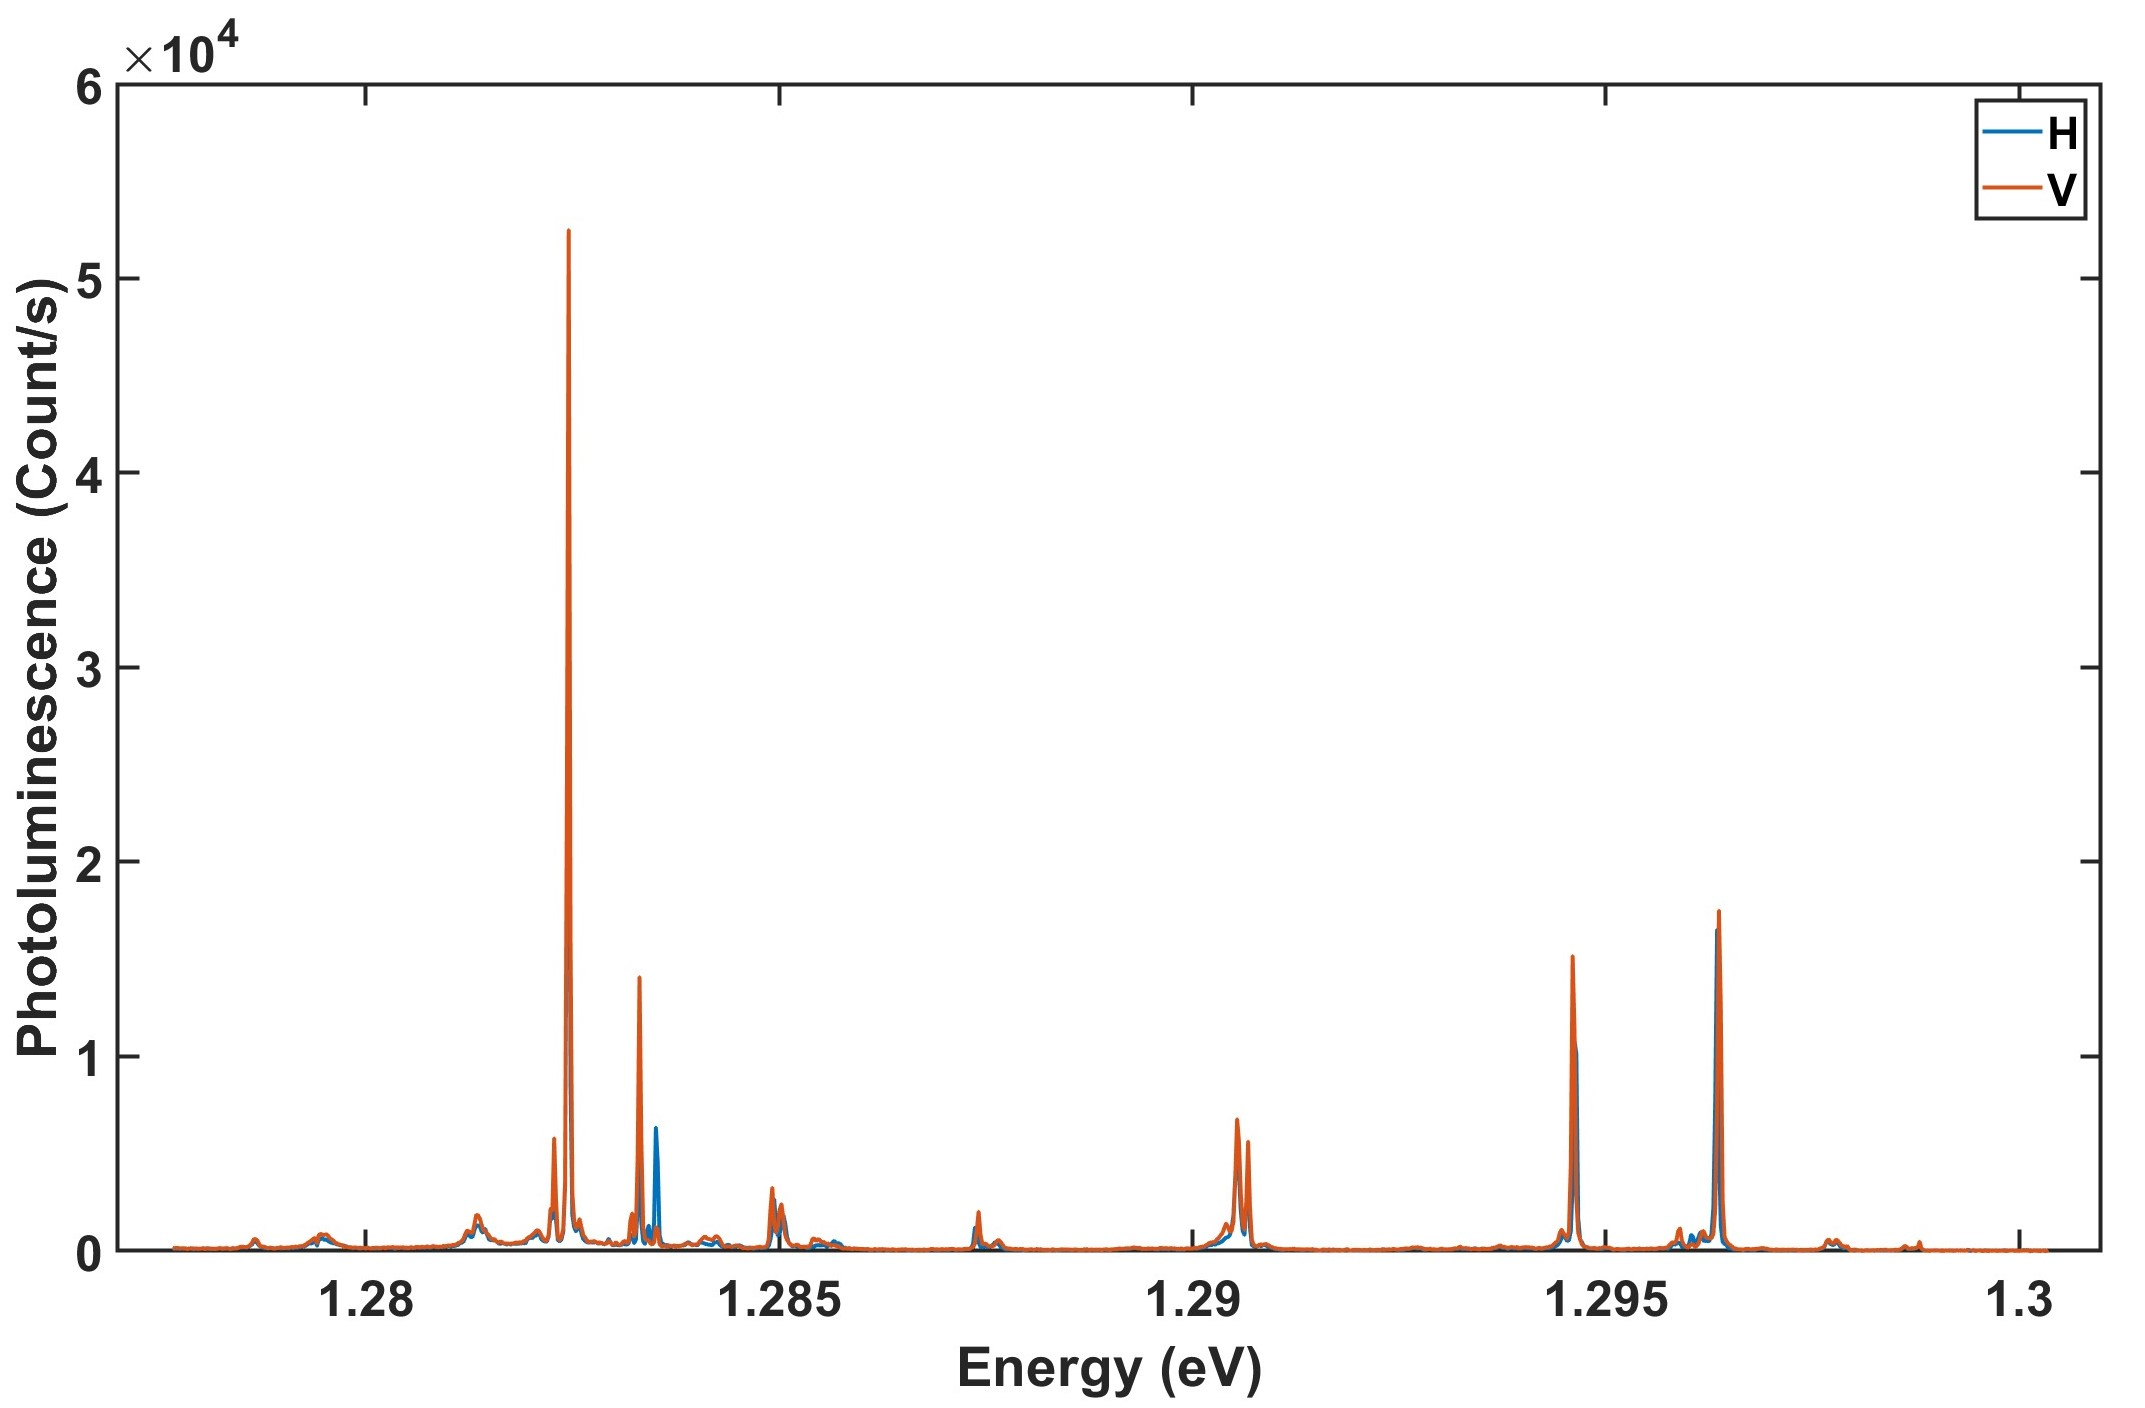
\includegraphics[scale=0.3]{figures/Spectrum.jpg}
		\caption{Polarization dependent photoluminescence spectra from a single quantum dot in a microcavity.}
		\label{fig:Spectrum_HV}
	\end{figure}
\subsection{Photoluminescence Spectroscopy}
\subsection{Exciton-biexciton cascade under CW excitation}
\begin{figure}[H]
	\centering
	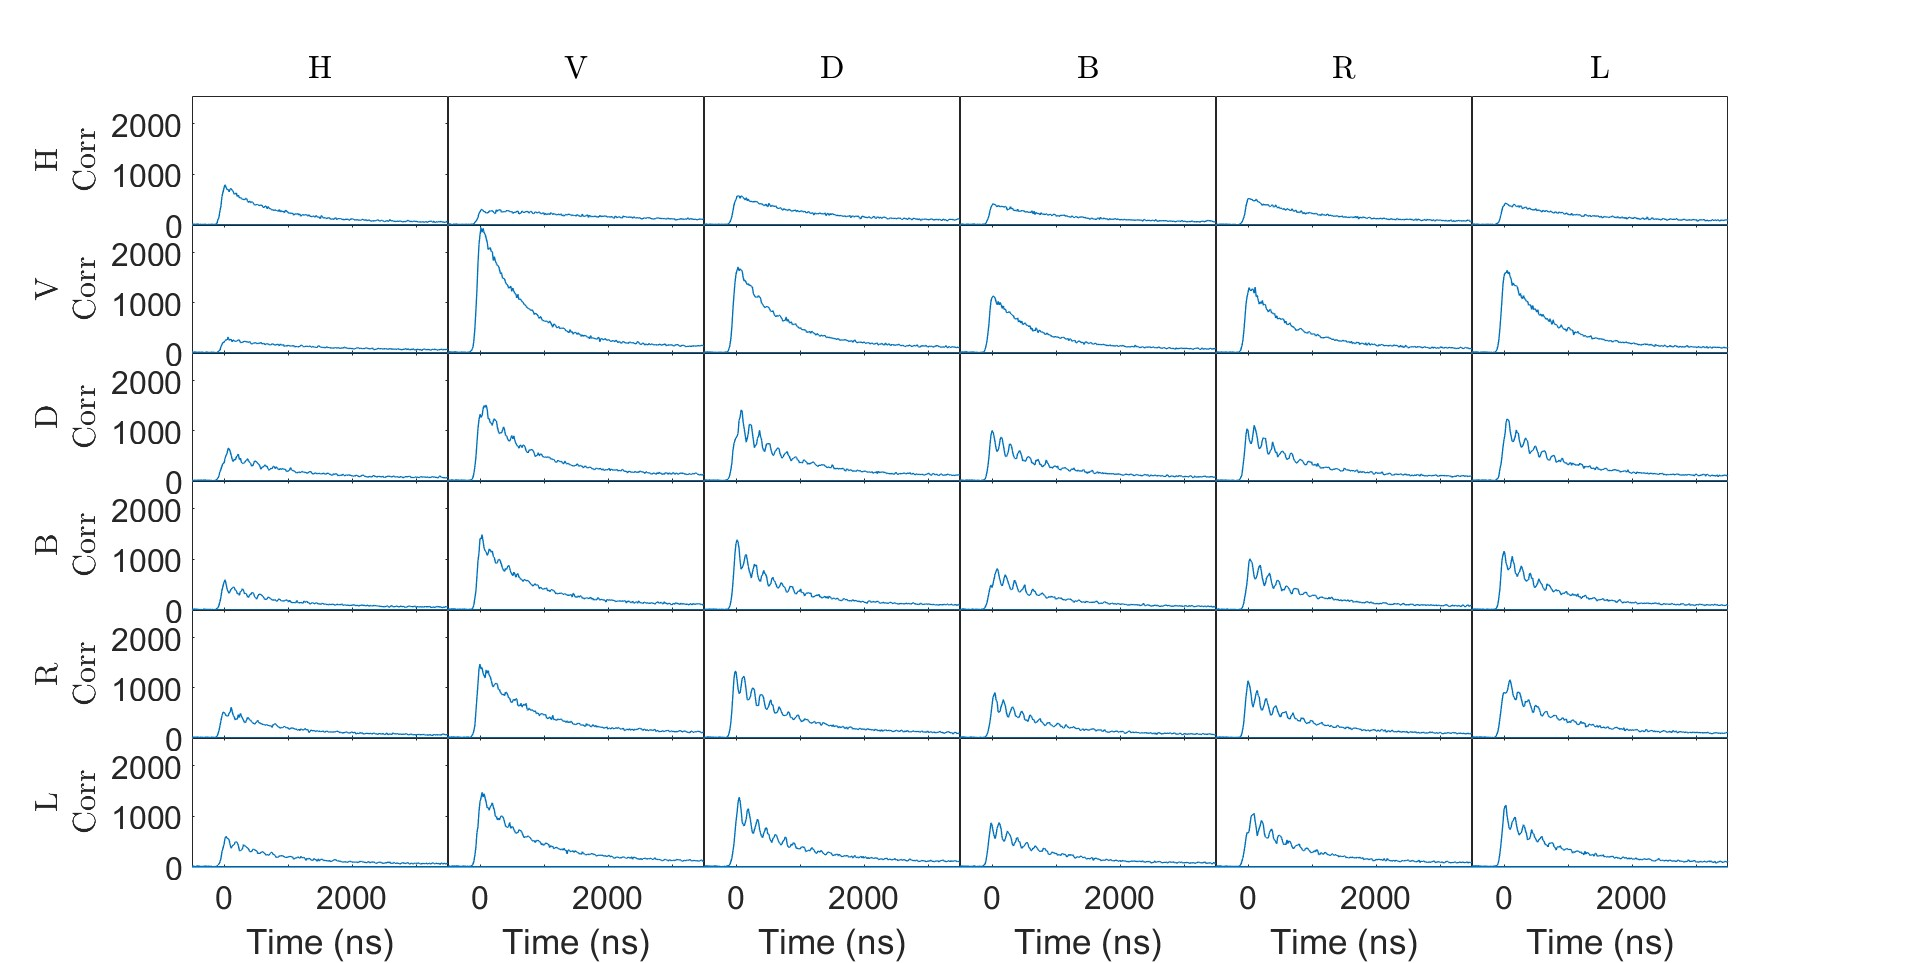
\includegraphics[scale=0.24]{figures/XX_X_Correlations.jpg}
	\caption{ Correlations of the biexciton-exciton radiative cascade., where each row (column) represents a biexciton (exciton) photon polarization (H,V,D,B,R,L).}
	\label{fig:PiSystem}
\end{figure}
\subsection{Exciton-biexciton cascade under pulsed excitation}
\subsection{Mach-Zender Interferometer}
The Mach-Zehnder interferometer consists of a light source that produces a coherent beam of light, which is then split into two separate paths by a beam splitter. Each path contains a series of mirrors reflecting the light back toward the beam splitter. The two reflected beams are recombined at the beam splitter and directed toward a detector.\\
When the two beams are in phase, they will constructively interfere and produce a bright spot on the detector. When they are out of phase, they will destructively interfere and produce a dark spot. By varying the path length of one of the arms of the interferometer, the relative phase between the two beams can be changed, causing the interference pattern to shift from bright to dark or vice versa.
\subsubsection{Schematic}

\subsubsection{Measurements of stability}
\begin{figure}[H]
	\centering
	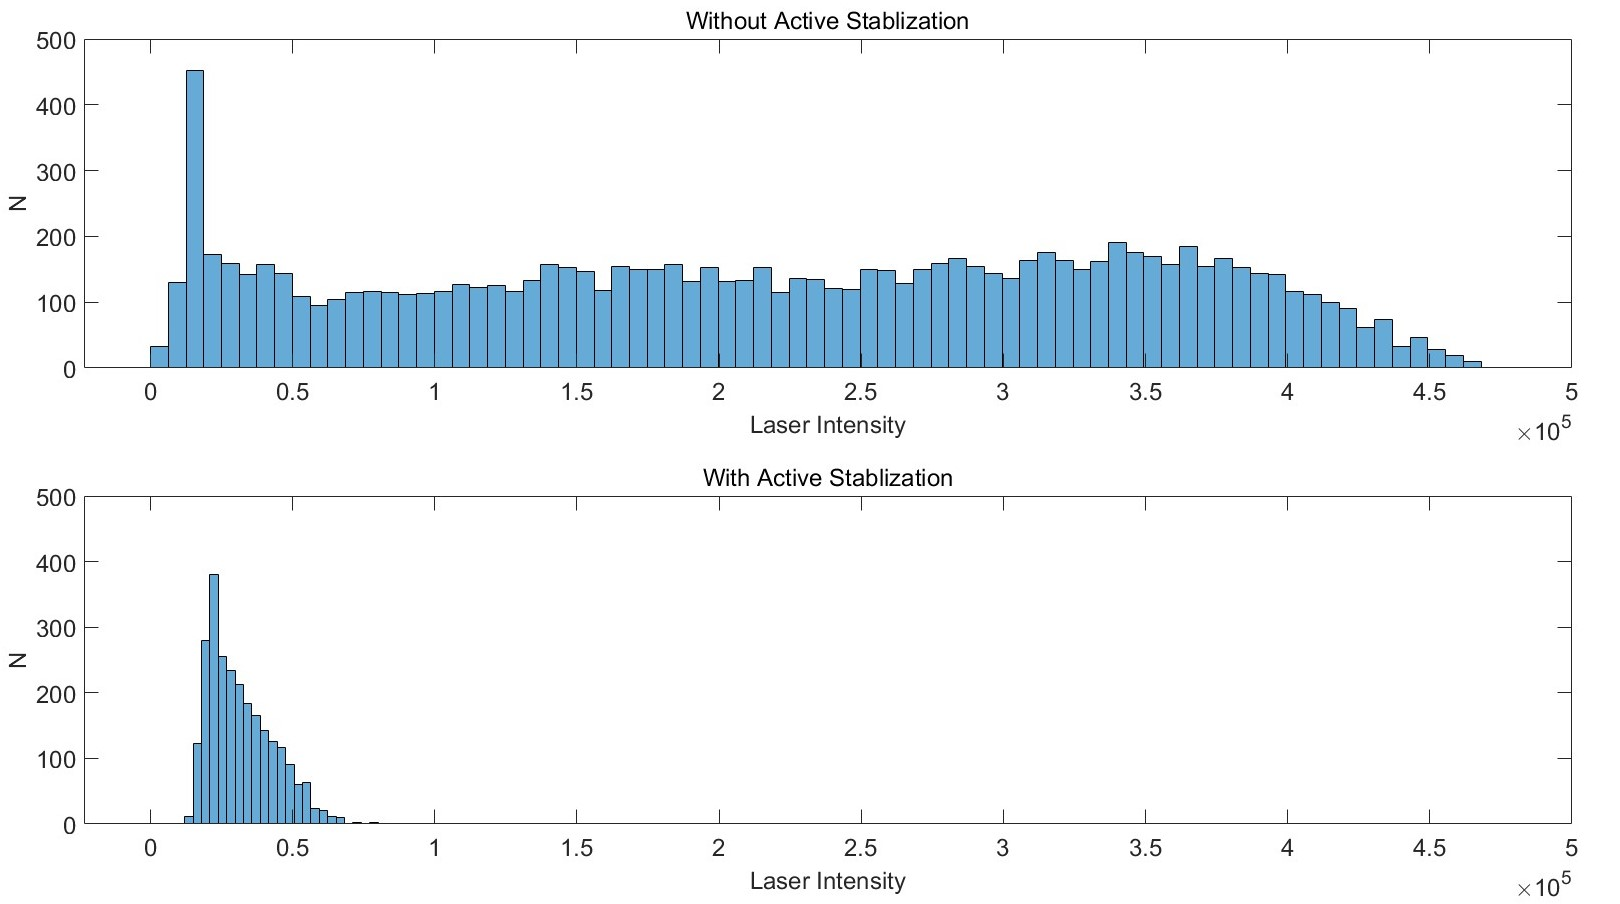
\includegraphics[scale=0.32]{figures/StablizationHistogram.jpg}
	\caption{Schematic description of the bright and dark exciton energy levels and spin eigenstates. The polarization of light that interacts with the BE eigenstates is marked underneath the corresponding BE eigenstate.}
	\label{fig:stablization_histogram}
\end{figure}
\subsection{Experimental setup}
	\begin{figure}[H]
		\centering
		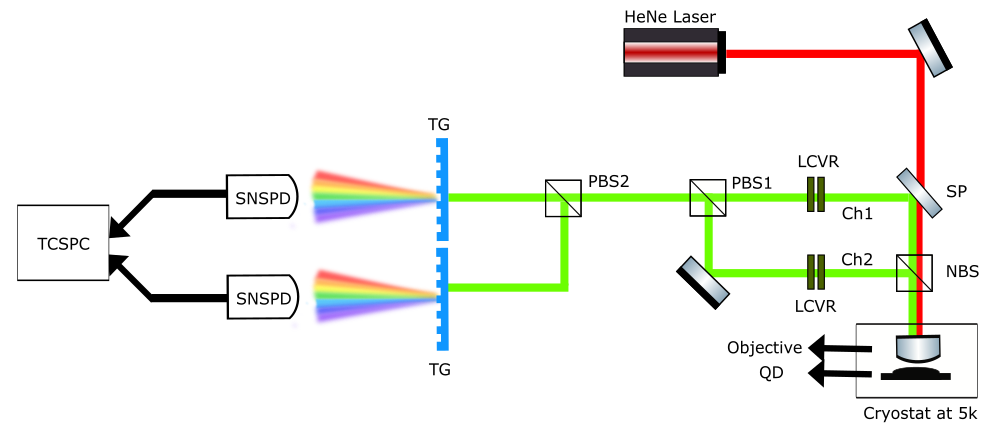
\includegraphics[scale=0.60]{figures/Experiment_schematics.png}
		\caption{Schematics of the measurement setup.}
		\label{fig:experiment_schematics}
	\end{figure}
Figure \ref{fig:experiment_schematics}  is a schematic of the experimental setup. The sample is held in a cryostat  at a temperature of 5K. The PL is collected using an objective lens with a numerical aperture of 0.85. The same objective also focuses the exciting lasers into the sample. We used a tunable, $76\,\rm MHz$ pulsed laser for the lifetime measurement and a CW, $632.8\,\rm nm$ HeNe laser, to perform the correlation measurements. \\
The PL collected from the dot is split into two channels using a non-polarizing beamsplitter (BS), wherein one of the channels, a short pass filter (LP), is used for transmitting the laser while reflecting the PL.\\
In both channels, the PL passes through a liquid crystal variable retarder (LCVR), which projects its polarization onto the axis of the first polarized beam splitter (PBS), where both channels recombine such as the H(V) polarization of the first(second) channel combine with the V(H) polarization from the second(first) channel and vice versa. Finally, the PL reaches the transmission grating (TG), where the PL is dispersed, and only photons with specific energy reach the superconducting nanowire single photon detector (SNSPD). The signal emitted from the detector is sent to a time-correlated single photon counter (TCSPC) that registers the time information about the events and saves it for analysis. 


